\section{Classi principali del modello logico}

\begin{figure}[H]
    \begin{adjustwidth}{-2cm}{-2cm}
        \centering
        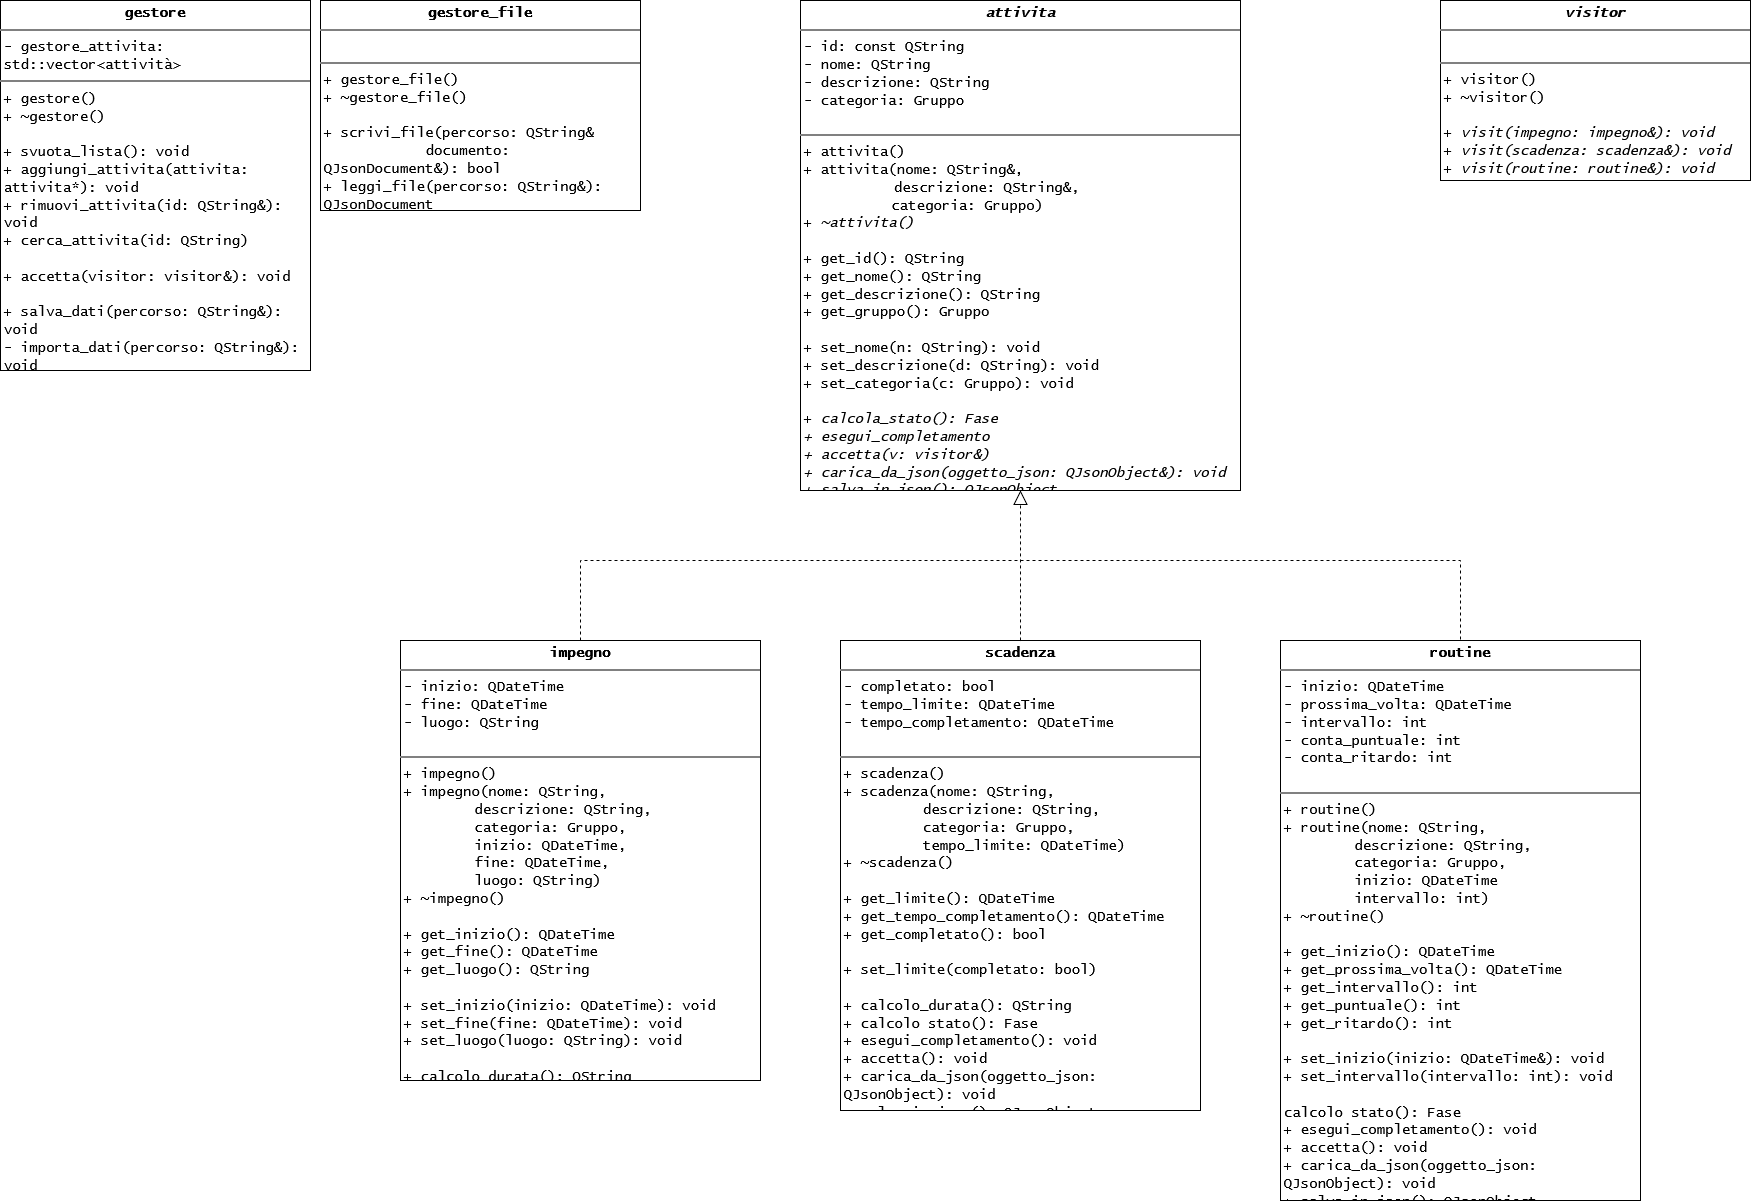
\includegraphics[width=1.25\textwidth, keepaspectratio]{allegati/uml_modello.drawio.png}
        \caption{Schema UML del modello logico}
        \label{fig:er-diagram}
    \end{adjustwidth}
\end{figure}

Per migliorare l'estensibilità del progetto, si è scelto di applicare
il design pattern architetturale MVC (Model-View-Controller), che
permette la separazione della logica dall'interfaccia grafica. In tale
contesto, la gestione delle caratteristiche funzionali delle attività è
affidata al Model.

Il fondamento dell'architettura è la classe base astratta \texttt{attivita}, che
presenta le caratteristiche base di ogni tipo di attività, come titolo, descrizione e
categoria di appartenenza.
Da essa derivano le classi concrete, cioè tipologie di attività con attributi strutturali
e comportamentali differenti tra loro. Attualmente, si è deciso di implementare le seguenti
categorie:
\begin{itemize}
    \item \textbf{Impegno}: caratterizzato da un inizio, una fine e il luogo in cui avviene.
    Non prevede un completamento, dato che si presuppone completato dopo la fine dell'impegno.
    \item \textbf{Scadenza}: non prevede un'inizio o una fine, ma solamente un limite e un
    tempo di completamento. Grazie a questi due elementi, diventa possibile tenere traccia
    dell'eventuale ritardo nel completamento della scadenza.
    \item \textbf{Routine}: non è caratterizzata da un tempo limite o di fine, ma è un'attività
    che si ripete indefinitamente. Impostando il tempo di inizio e l'intervallo, il sistema calcola
    automaticamente il termine della prossima iterazione della routine. Il sistema permette
    anche il numero di volte in cui è stata completata l'iterazione, tenendo anche traccia di
    puntualità e ritardi.
\end{itemize}

La gestione vera e propria delle instanze delle classi è affidata alla classe \texttt{gestore},
che, tramite un \texttt{std::vector<attivita*>} permette all'applicazione di effettuare le
operazioni CRUD. I vantaggi dell'uso di puntatori alla classe astratta \texttt{attivita} sono
la possibilità di implementare il polimorfismo e il rispetto del principio Open-Closed:
è possibile, infatti, inserire altre classi derivate concrete senza necessità di modificare
il codice del gestore.

Si è scelto di usare un \texttt{std::vector} per sfruttare la proprietà di continuità dei vettori:
infatti, le operazioni effettuate più frequentemente sono l'accesso arbitrario (visualizzazione e
modifica di un'attività) e l'accesso in serie (il refresh dell'intero elenco visivo in seguito a
modifiche o eliminazioni).

Il \texttt{gestore} contiene anche un \texttt{gestore\_file}, che si occupa esclusivamente della
persistenza delle attività.

Infine, il Model contiene la classe astratta \texttt{visitor}, da cui derivano i vari visitor usati
all'interno del programma per semplificare il codice grazie all'applicazione del polimorfismo.